\documentclass[11pt, a4paper]{article}
\usepackage{pdfpages}
\usepackage{parallel}
\usepackage[T2A]{fontenc}
%\usepackage{ucs}
\usepackage[utf8]{inputenc}
\usepackage[english,russian]{babel}
\usepackage{hyperref}
\usepackage{rotating}
\usepackage[inner=2cm,top=1.8cm,outer=2cm,bottom=2.3cm,nohead]{geometry}
%\usepackage{listings}
\usepackage{graphicx}
\usepackage{wrapfig}
\usepackage{longtable}
\usepackage{indentfirst}
\usepackage{array}
\usepackage{tikzsymbols}
\usepackage{soul}
\usepackage[ruled,vlined]{algorithm2e}
\usepackage{qrcode}
\counterwithout{figure}{section} 

\usepackage{url}
\makeatletter
\g@addto@macro{\UrlBreaks}{\UrlOrds}
\makeatother

\newcolumntype{P}[1]{>{\raggedright\arraybackslash}p{#1}}
\frenchspacing
%\usepackage{fixltx2e} %text sub- and superscripts
\usepackage{icomma} % коскі ў матэматычным рэжыме
%\PreloadUnicodePage{4}

\newcommand{\longpage}{\enlargethispage{\baselineskip}}
\newcommand{\shortpage}{\enlargethispage{-\baselineskip}}

\def\switchlang#1{\expandafter\csname switchlang#1\endcsname}
\def\switchlangbe{
\let\saverefname=\refname%
\def\refname{Літаратура}%
\def\figurename{Іл.}%
}
\def\switchlangru{
\let\saverefname=\refname%
\let\savefigurename=\figurename%
\def\refname{Литература}%
\def\figurename{Рис.}%
}
\def\switchlangen{
\let\saverefname=\refname%
\def\refname{References}%
\def\figurename{Fig.}%
}

\hyphenation{admi-ni-stra-tive}
\hyphenation{ex-pe-ri-ence}
\hyphenation{fle-xi-bi-li-ty}
\hyphenation{Py-thon}
\hyphenation{ma-the-ma-ti-cal}
\hyphenation{re-ported}
\hyphenation{imp-le-menta-tions}
\hyphenation{pro-vides}
\hyphenation{en-gi-neering}
\hyphenation{com-pa-ti-bi-li-ty}
\hyphenation{im-pos-sible}
\hyphenation{desk-top}
\hyphenation{elec-tro-nic}
\hyphenation{com-pa-ny}
\hyphenation{de-ve-lop-ment}
\hyphenation{de-ve-loping}
\hyphenation{de-ve-lop}
\hyphenation{da-ta-ba-se}
\hyphenation{plat-forms}
\hyphenation{or-ga-ni-za-tion}
\hyphenation{pro-gramming}
\hyphenation{in-stru-ments}
\hyphenation{Li-nux}
\hyphenation{sour-ce}
\hyphenation{en-vi-ron-ment}
\hyphenation{Te-le-pathy}
\hyphenation{Li-nux-ov-ka}
\hyphenation{Open-BSD}
\hyphenation{Free-BSD}
\hyphenation{men-ti-on-ed}
\hyphenation{app-li-ca-tion}

\def\progref!#1!{\texttt{#1}}
\renewcommand{\arraystretch}{2} %Іначай формулы ў матрыцы зліпаюцца з лініямі
\usepackage{array}

\def\interview #1 (#2), #3, #4, #5\par{

\section[#1, #3, #4]{#1 -- #3, #4}
\def\qname{LVEE}
\def\aname{#1}
\def\q ##1\par{{\noindent \bf \qname: ##1 }\par}
\def\a{{\noindent \bf \aname: } \def\qname{L}\def\aname{#2}}
}

\def\interview* #1 (#2), #3, #4, #5\par{

\section*{#1\\{\small\rm #3, #4. #5}}
\ifx\ParallelWhichBox\undefined%
    \addcontentsline{toc}{section}{#1, #3, #4}%
\else%
\ifnum\ParallelWhichBox=0%
    \addcontentsline{toc}{section}{#1, #3, #4}%
\fi\fi%

\def\qname{LVEE}
\def\aname{#1}
\def\q ##1\par{{\noindent \bf \qname: ##1 }\par}
\def\a{{\noindent \bf \aname: } \def\qname{L}\def\aname{#2}}
}

\newcommand{\interviewfooter}[1]{
\vskip 1em
\noindent \textit{#1}
}

\AtEndDocument{\vfill\centering \qrcode{https://github.com/fiowro/mouses/blob/main/\jobname.pdf}}

\switchlang{ru}
\begin{document}

\title{1981 "--- Xerox Alto Optical Mouse}
\date{}
\maketitle
\selectlanguage{russian}
В сентябре 1986 года корпорация Xerox анонсировала рабочую станцию EWS 4800, работавшую под управлением ОС UNIX. Эта машина была спроектирована как рабочая станция для инженеров, для повышения эффективности решения таких задач, как разработка программного обеспечения, автоматизированное проектирование, научные и инженерные вычисления, сбор и анализ экспериментальных данных \cite{yt}. Она была оснащена графическим многооконным интерфейсом и большим 20-дюймовым дисплеем разрешения $1280 \times 1024 \times 256$. В комплекте с этой мощной рабочей станцией поставлялась мышь Xerox Alto Mouse (рис. \ref{fig:XeroxAltoPic}).

Специально изготовленная микросхема и другие части были встроены в стандартный корпус мыши Xerox Alto \cite{vlsi82}.

\begin{figure}[h]
    \centering
    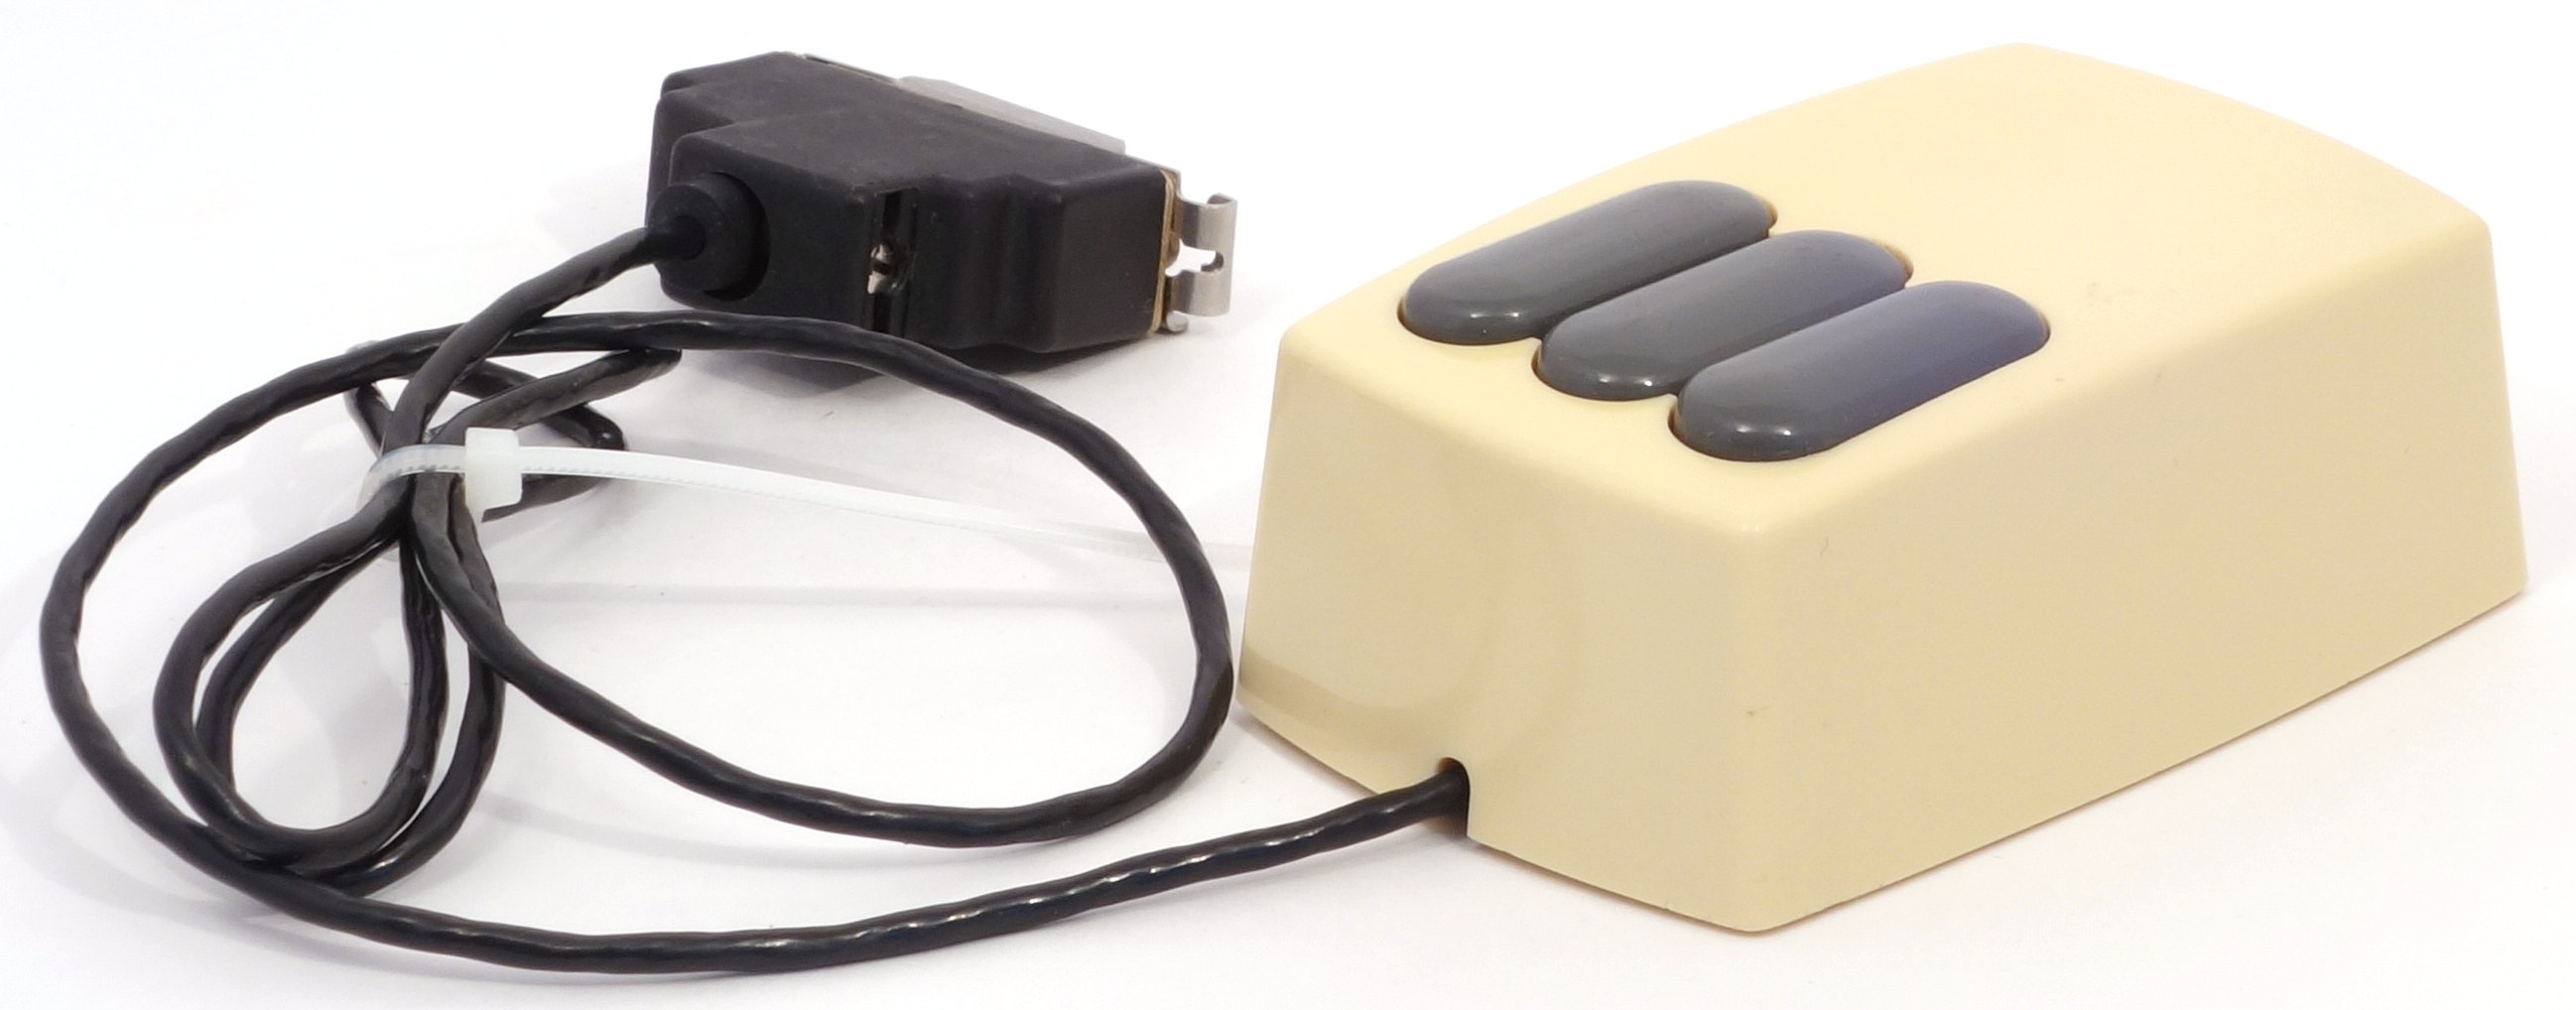
\includegraphics[scale=0.7]{1981_xerox_alto_mouse/pic_30.jpg}
    \caption{Xerox Alto Optical Mouse}
    \label{fig:XeroxAltoPic}
\end{figure}

Коврик для мыши был бумажным, продавался в пачках по 25 листов \cite{pad}. Узор представлял собой шестиугольный массив светлых точек на темном поле и был абсолютно пригоден для использования в случае его ксерокопирования. Реконструированный коврик можно увидеть на рис. \ref{fig:XeroxAltoPad}.

\begin{figure}[h]
    \centering
    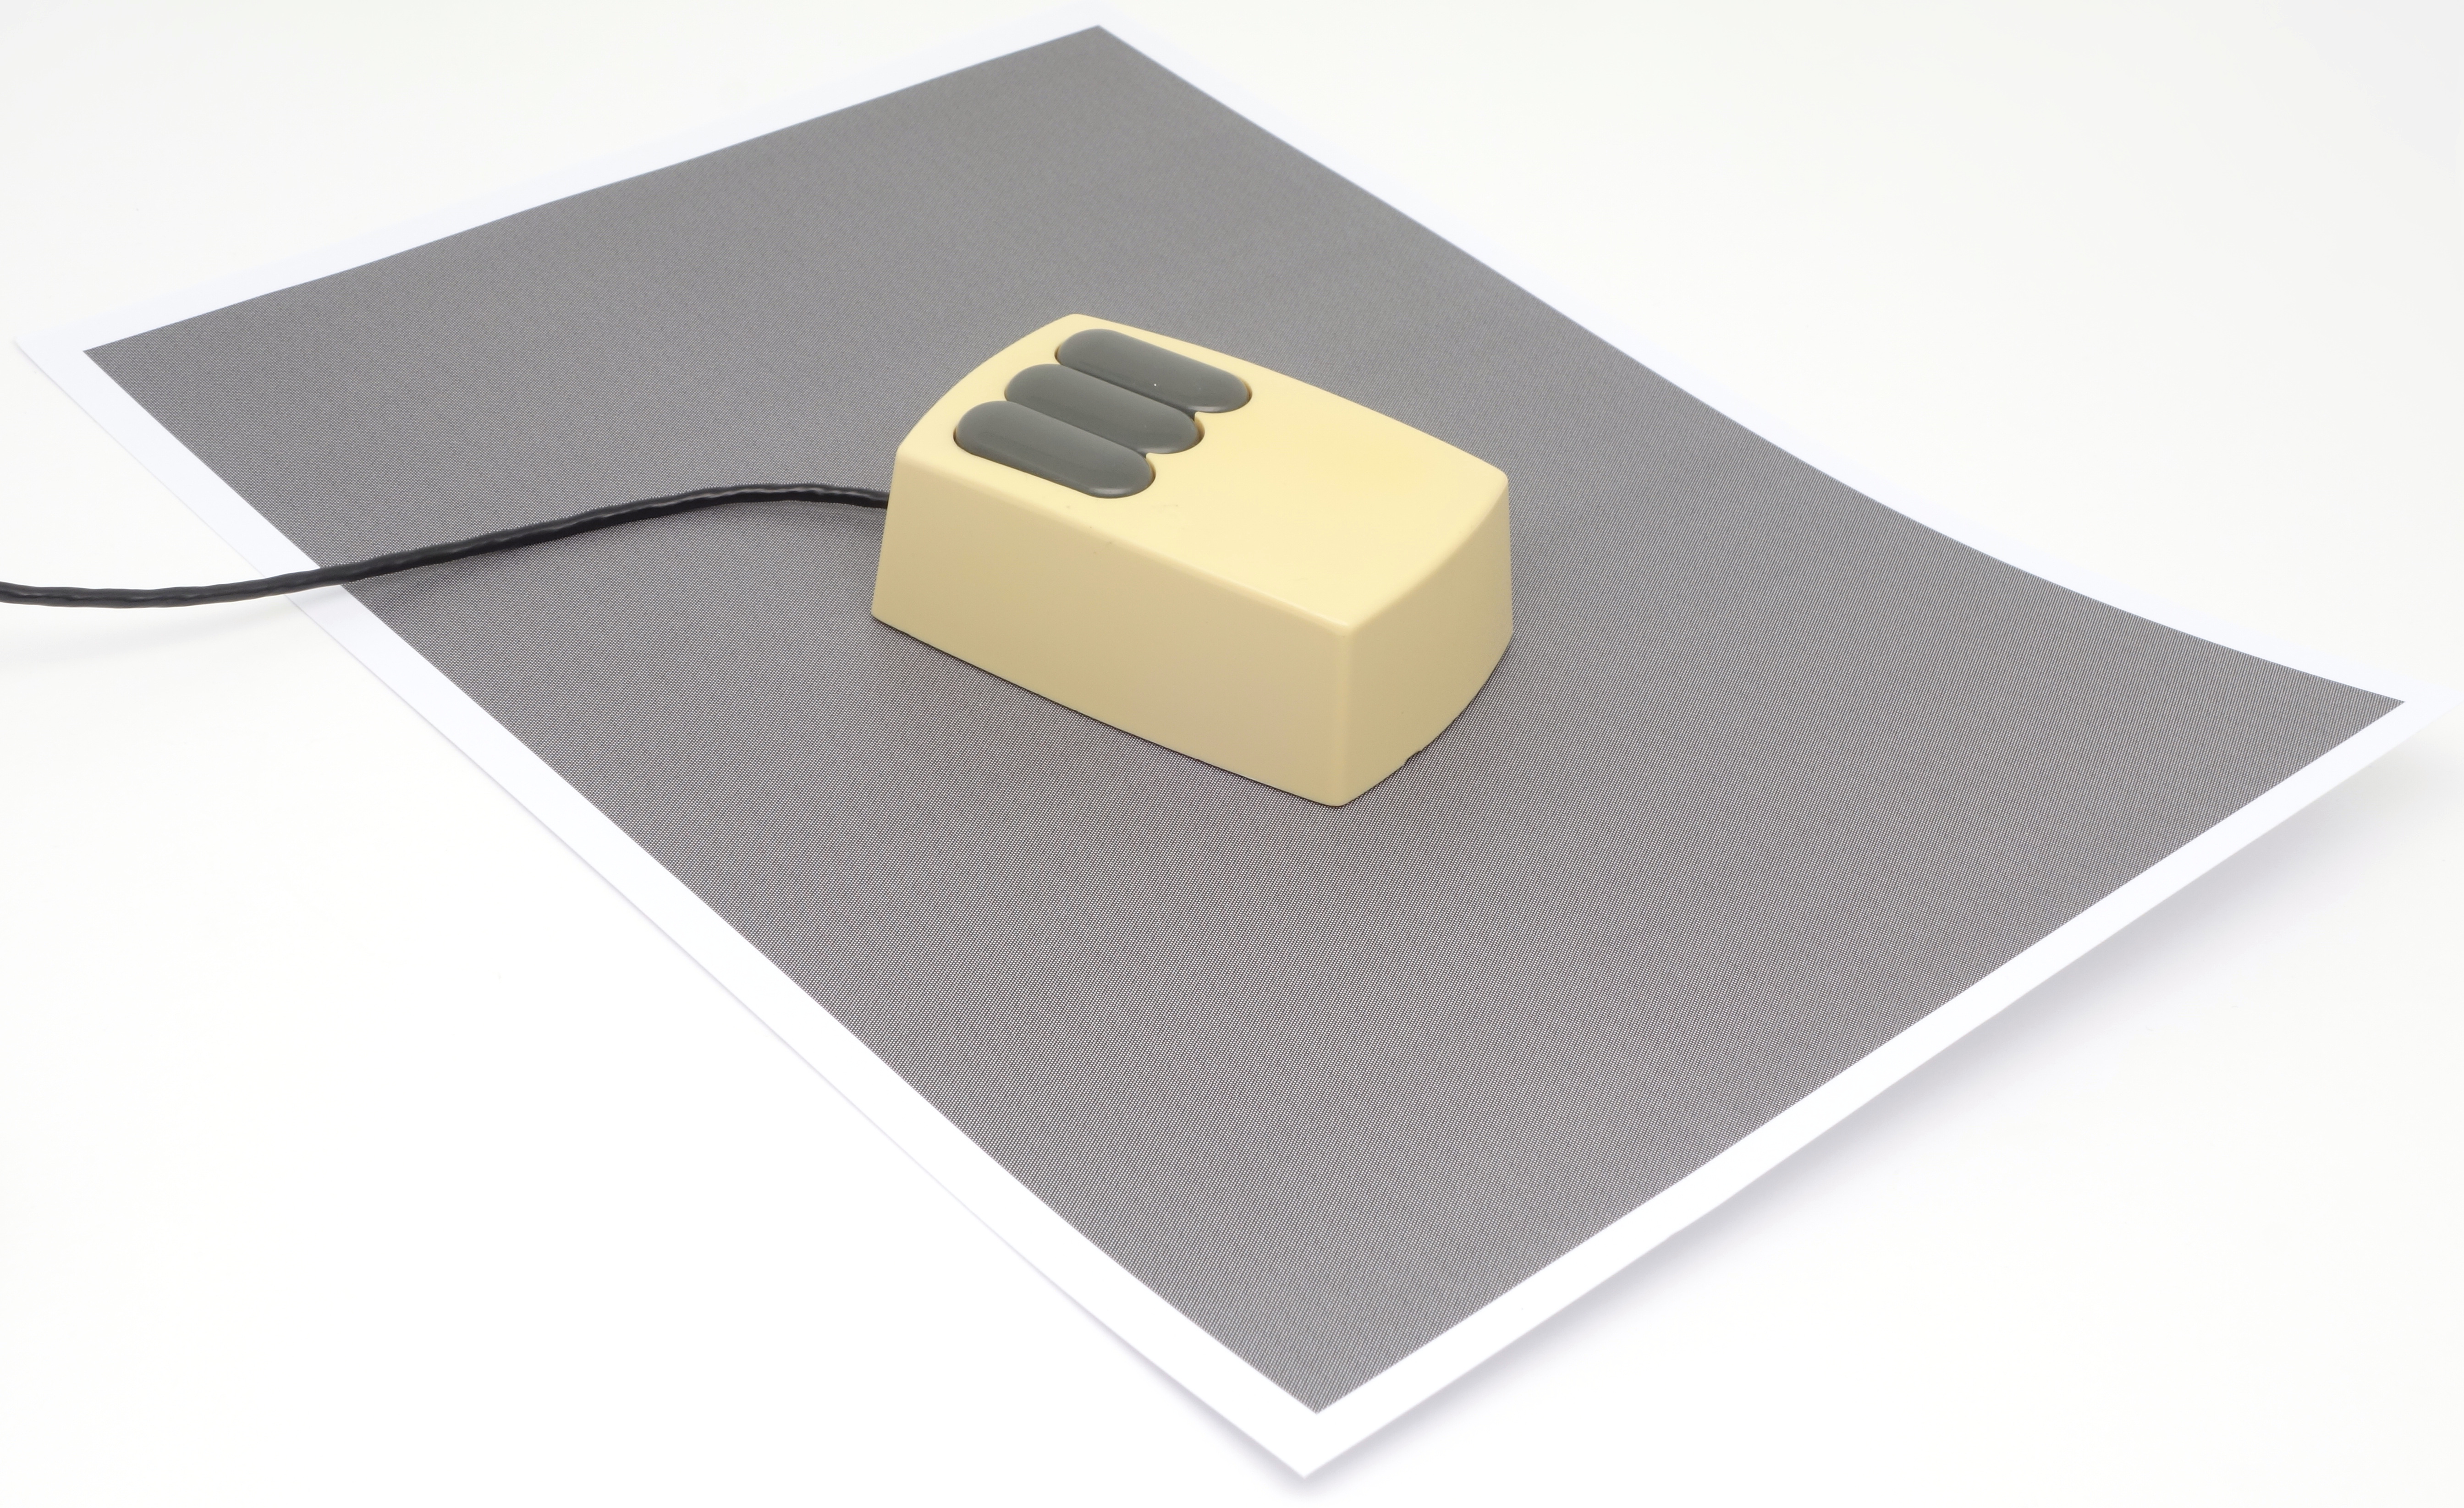
\includegraphics[scale=0.4]{1981_xerox_alto_mouse/pad_30.jpg}
    \caption{Xerox Alto Optical Mouse на реконструкции комплектного коврика}
    \label{fig:XeroxAltoPad}
\end{figure}

На верхней стороне корпуса выделено название мыши <<Alto Mouse>> с двумя треугольными стилизованными мышками в очертаниях и сплошных линиях. Нижняя сторона показывает, что это оптическая мышь (рис. \ref{NecAltoTopAndBottom}), во многом повторяющая внешние конструктивные решения мышей Mouse Systems того же периода и предназначенная для использования в комплекте со специальным зеркальным ковриком \cite{photo}.

\begin{figure}[h]
    \centering
    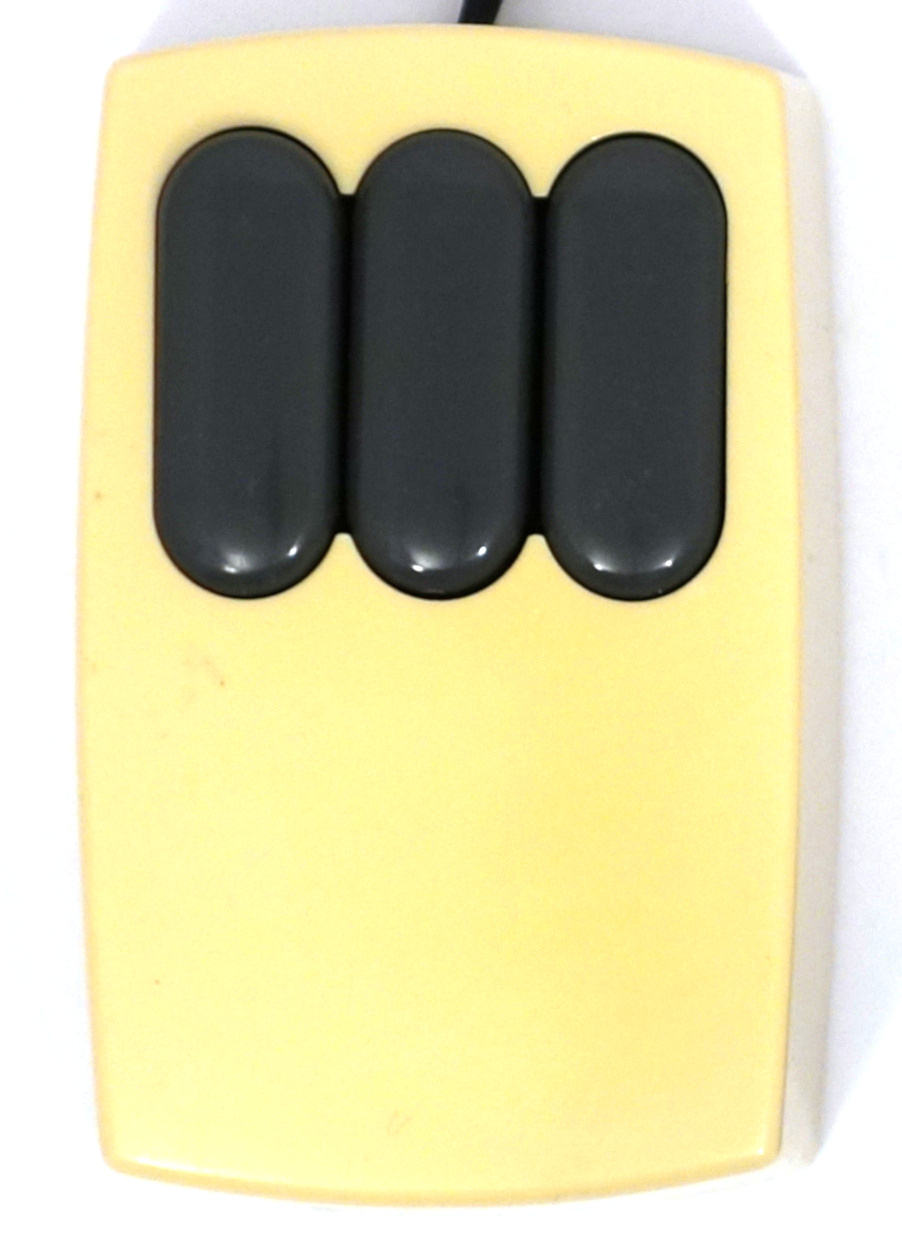
\includegraphics[scale=0.4]{1981_xerox_alto_mouse/top_30.jpg}
    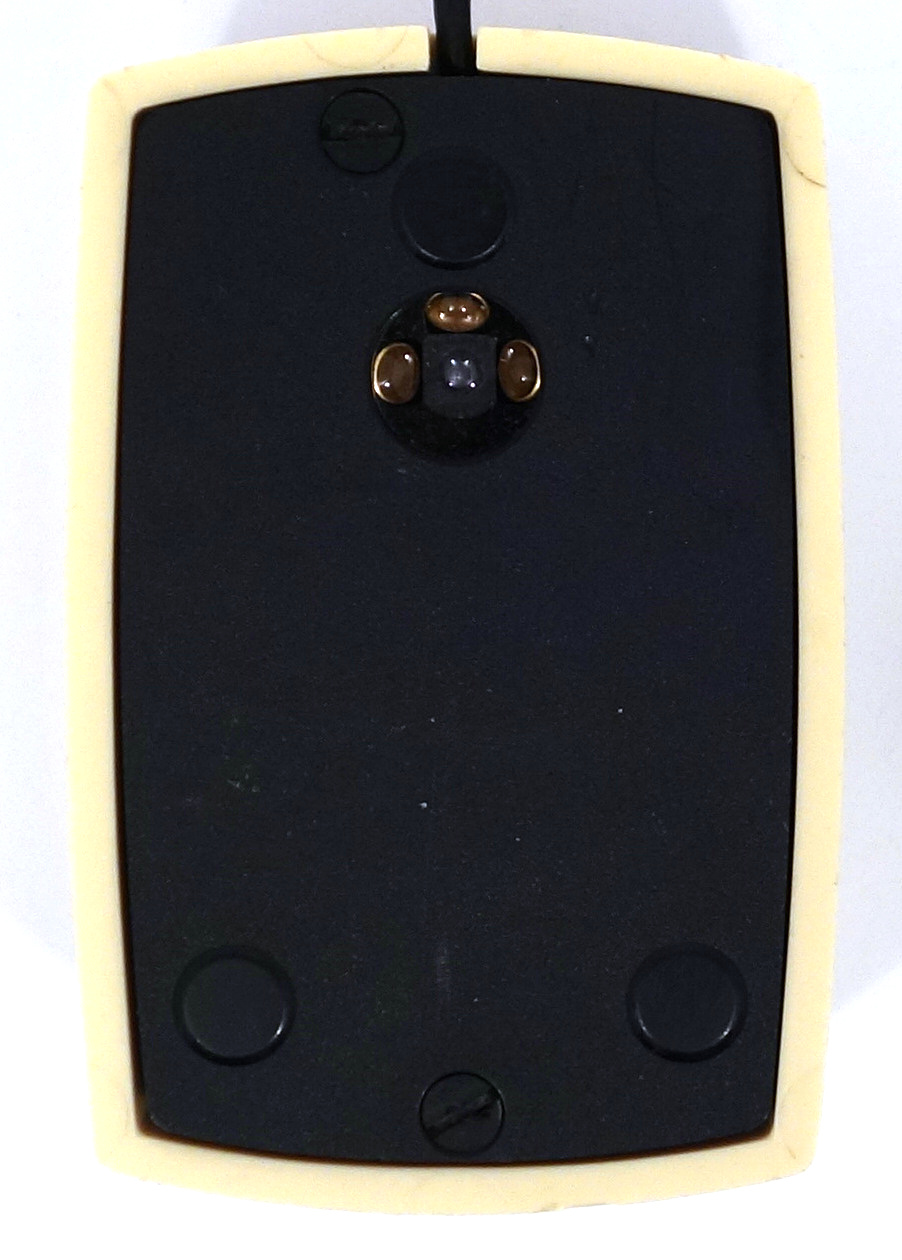
\includegraphics[scale=0.4]{1981_xerox_alto_mouse/bottom_30.jpg}
    \caption{Xerox Alto Optical Mouse, вид сверху и снизу}
    \label{NecAltoTopAndBottom}
\end{figure}

В плане размера манипулятор представляет собой типичное для 80-х годов оптическое устройство управления курсором (рис. \ref{fig:NecAltoSize})

\begin{figure}[h]
    \centering
    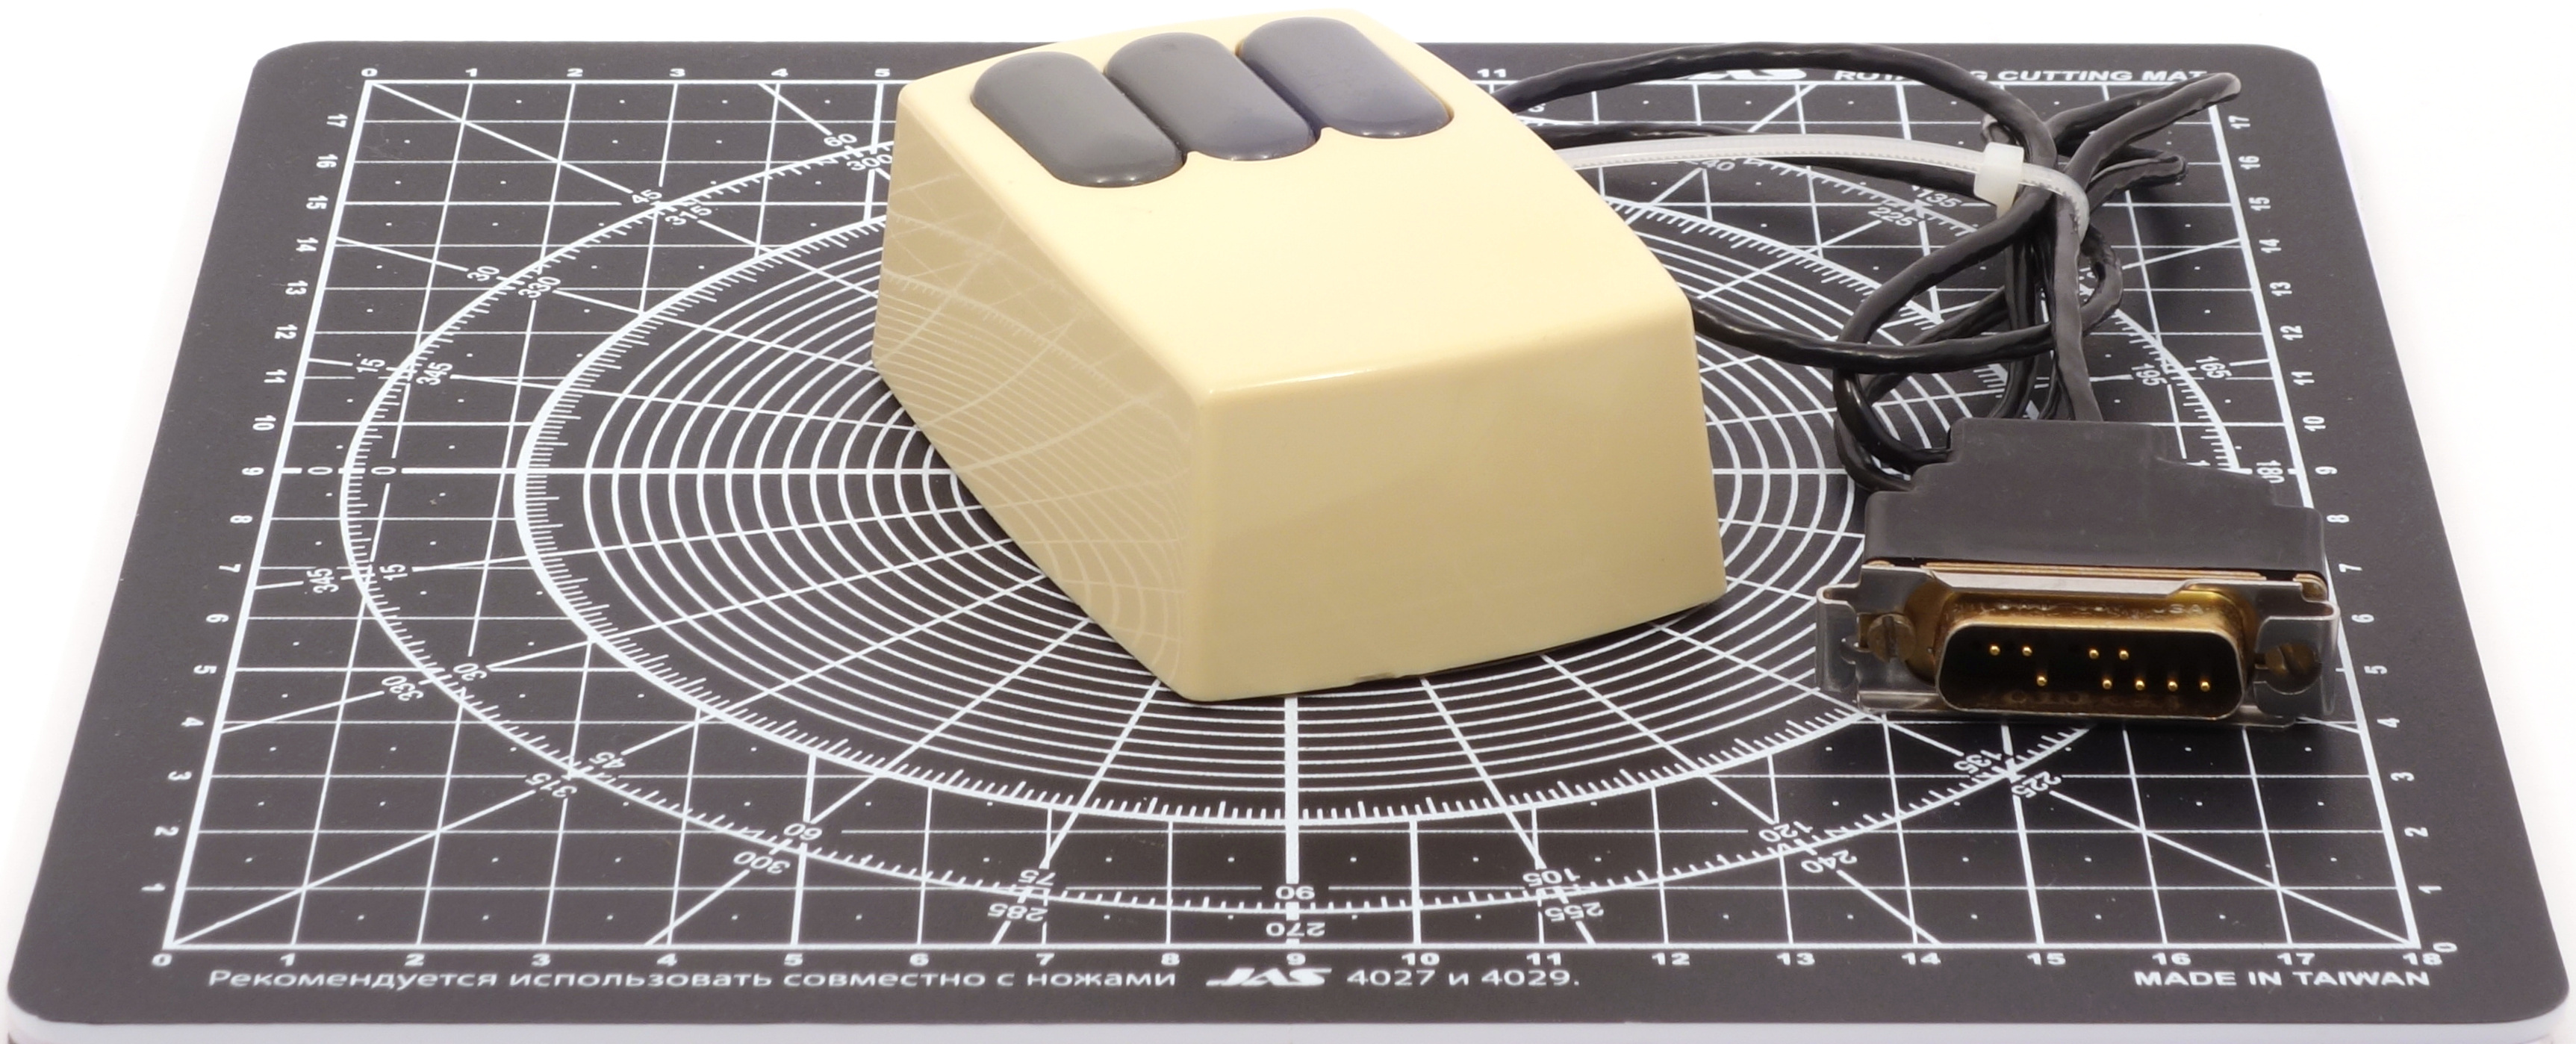
\includegraphics[scale=0.4]{1981_xerox_alto_mouse/size_15.jpg}
    \caption{Xerox Alto Optical Mouse на размерном коврике с шагом сетки 1~см}
    \label{fig:NecAltoSize}
\end{figure}

В плане эргономики во внешнем виде Alto Mouse прослеживается ярко выраженный индустриальный дизайн. При этом большое количество углов и плоских граней отчасти компенсируется закругленными стыками граней в ближней к пользователю части корпуса, и выпуклыми продолговатыми кнопками, удобно расположенными в зоне досягаемости пальцев (рис. \ref{fig:NecAltoHand}).

\begin{figure}[h]
    \centering
    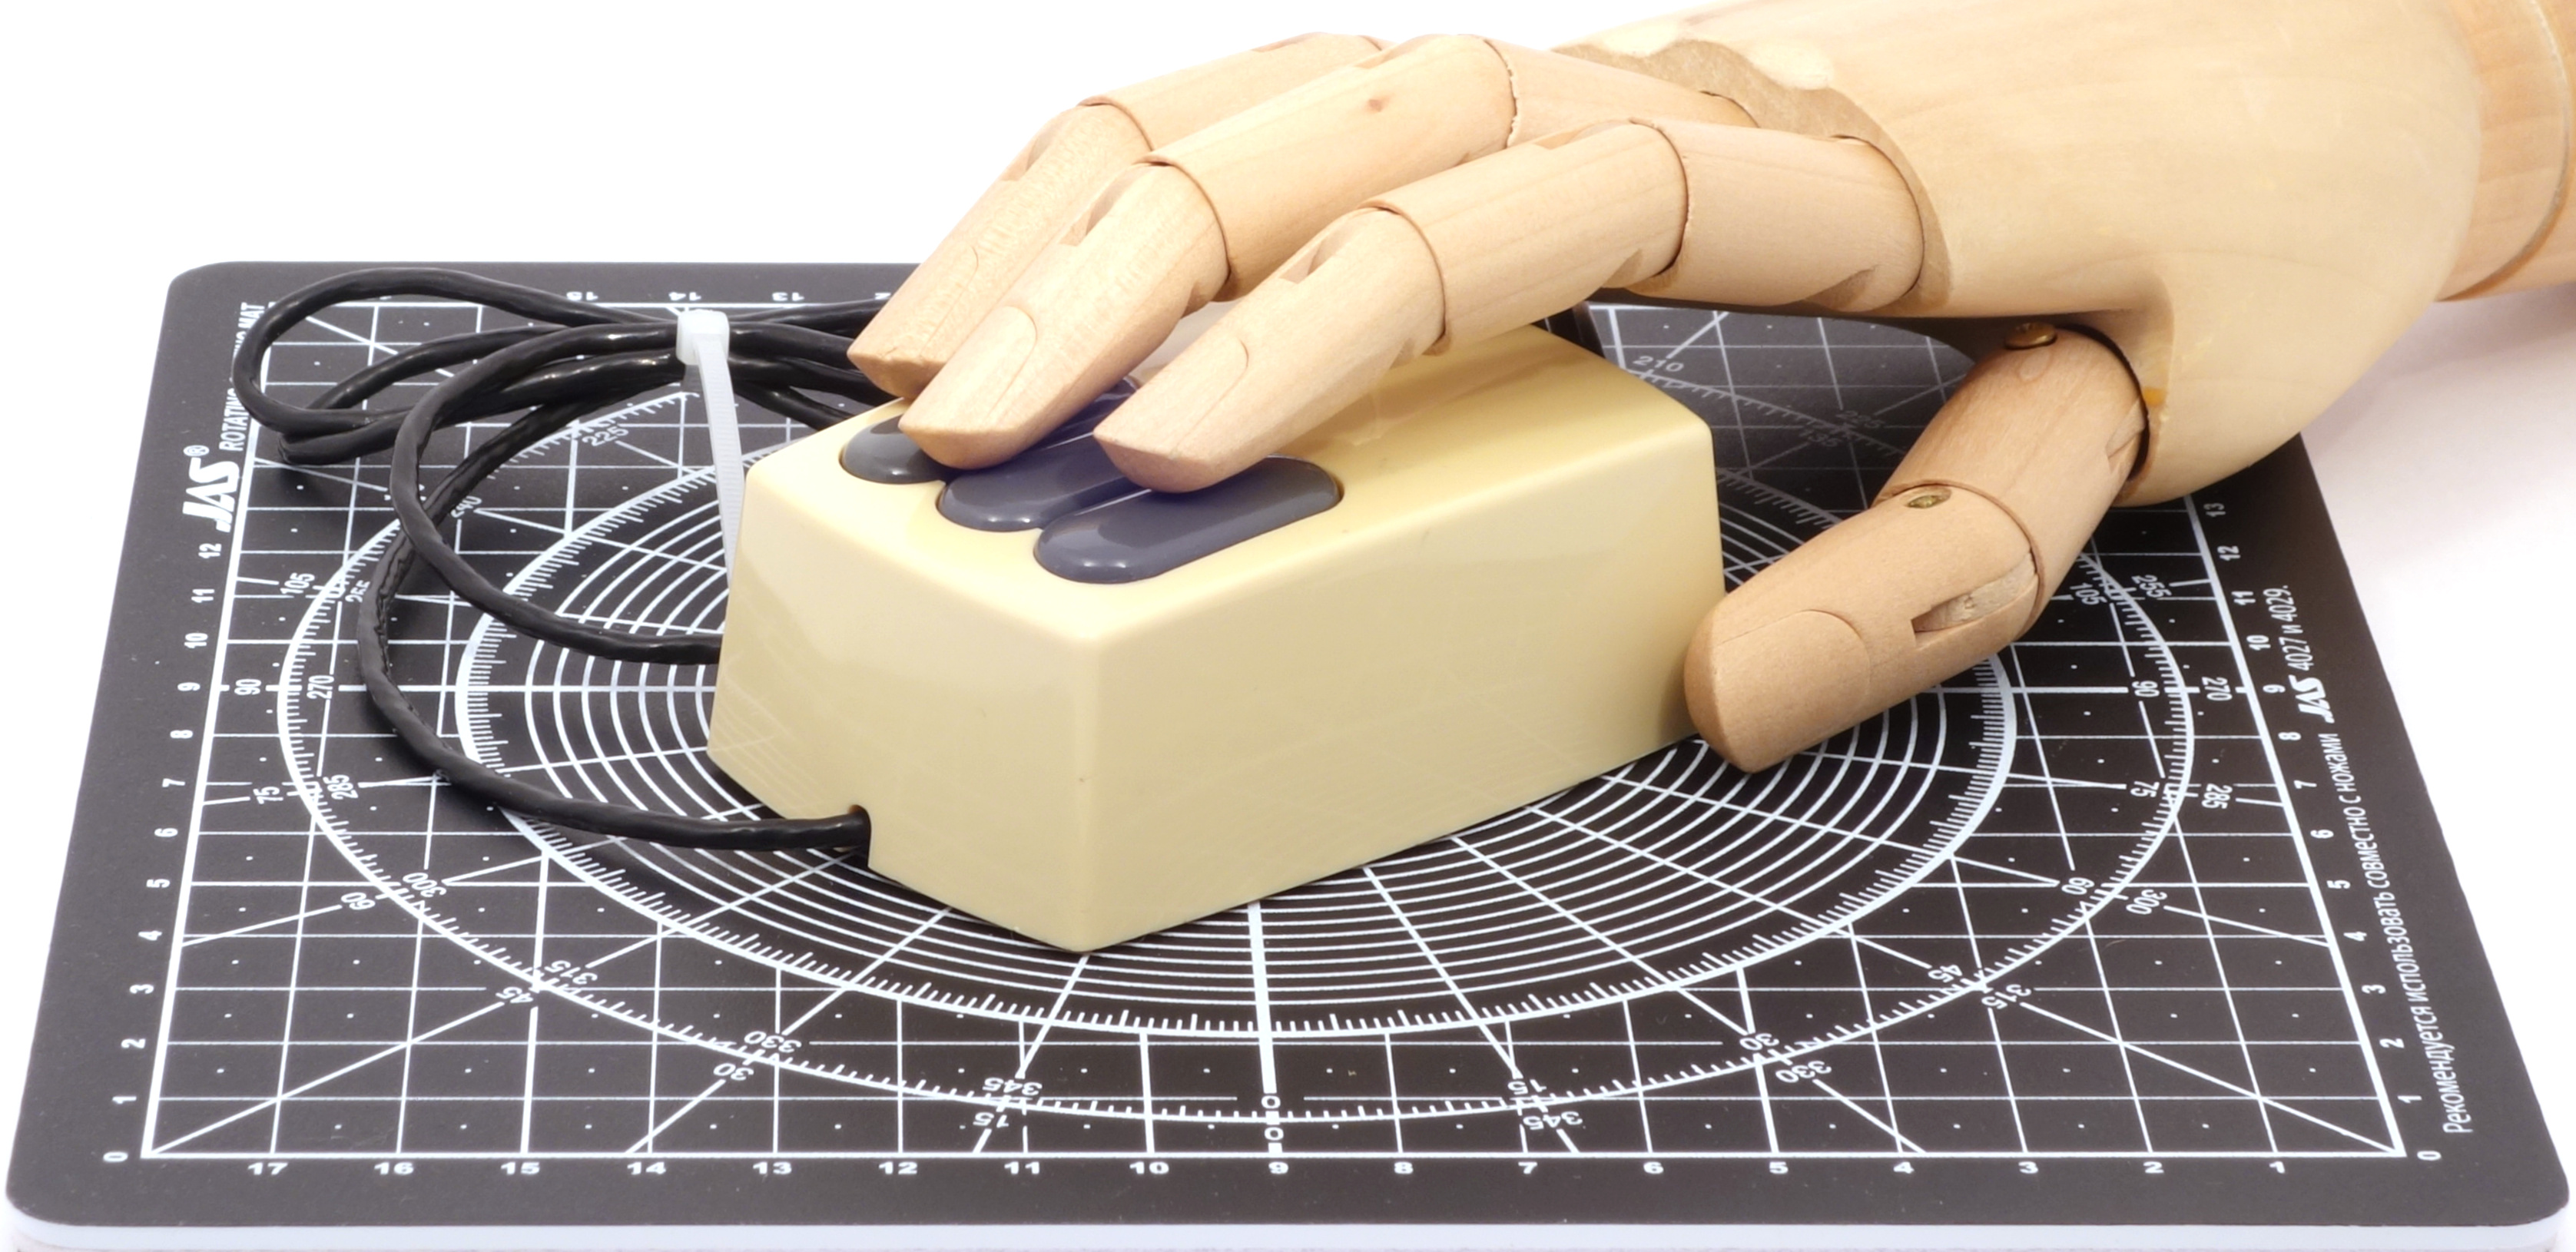
\includegraphics[scale=0.4]{1981_xerox_alto_mouse/hand_30.jpg}
    \caption{Xerox Alto Optical Mouse с моделью руки человека}
    \label{fig:NecAltoHand}
\end{figure}

Xerox Alto Mouse имеет разъём DIN и по интерфейсу подключения относится к категории Bus Mouse (шинная мышь). Особенностью таких мышей является то, что обработку сигналов оптопар производит не микросхема в корпусе мыши, а специальный адаптер в системном блоке компьютера; поэтому данная мышь питается от компьютера без отдельного блока питания, в отличие от многих ранних оптических моделей, подключавшихся к последовательному порту IBM PC.

\begin{figure}[h]
    \centering
    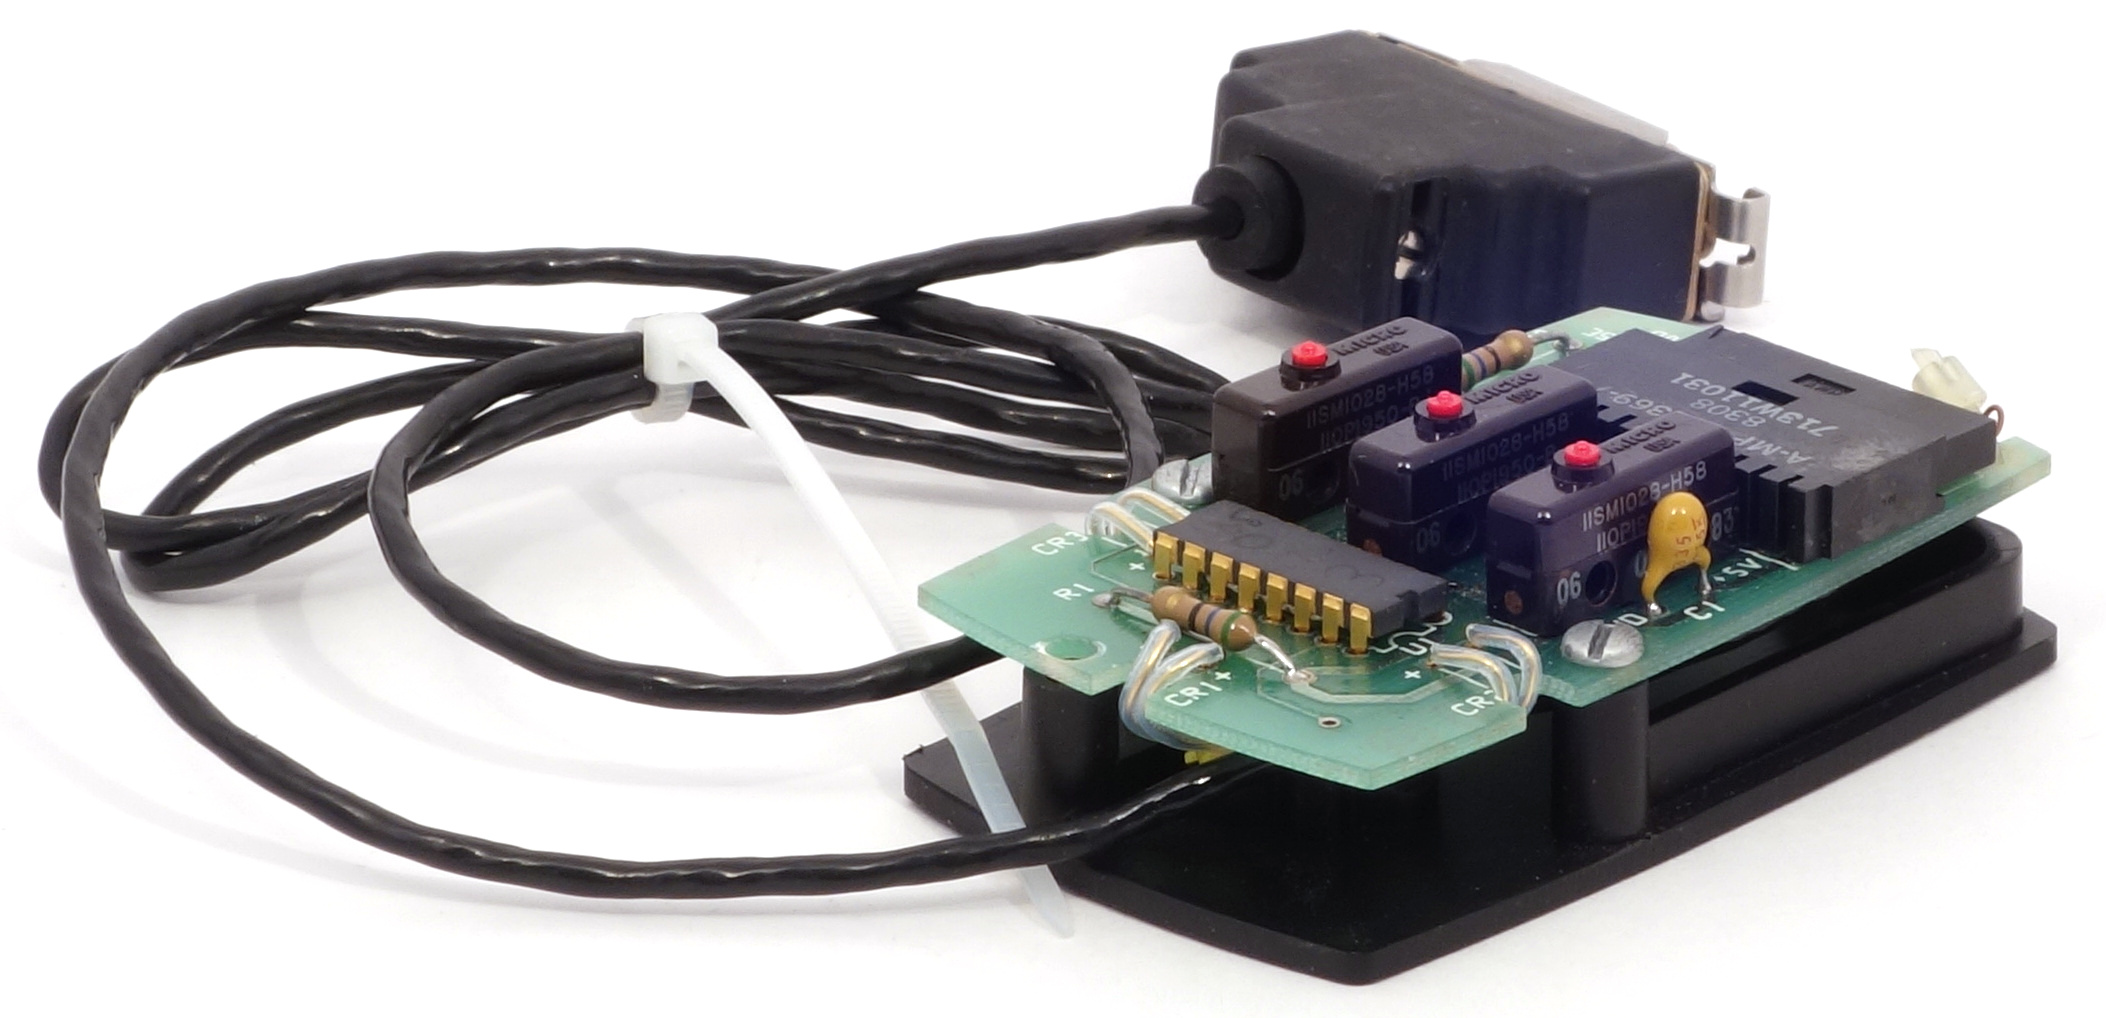
\includegraphics[scale=0.8]{1981_xerox_alto_mouse/inside_60.jpg}
    \caption{Xerox Alto Optical Mouse в разобранном виде}
    \label{fig:NecAltoInside}
\end{figure}

В разобранном виде манипулятор показан на рис. \ref{fig:NecAltoInside}, где можно увидеть оригинальную конструкцию оптической мыши, однако в отличие от большинства оптических мышей 80-х годов, не являющейся прямой копией изделия Mouse Systems, ставшей прототипом для последующих манипуляторов данного типа.
    
\begin{thebibliography}{9}
\bibitem {vlsi81} R.\,F. Lyon. The Optical Mouse, and an Architectural Methodology for
Smart Digital Sensors // VLSI DESIGN, August 1981. - p. 20--30. \url{https://www.dicklyon.com/tech/OMouse/OpticalMouse-Lyon.pdf}
\bibitem {vlsi82} R.\,F. Lyon, M.\,P. Haeberli. Designing and Testing The Optical Mouse // VLSI DESIGN, January/February, 1982. - p. 20--30. \url{https://www.dicklyon.com/tech/OMouse/DesigningTestingOMouse.pdf}
\bibitem{pad} R.\,F. Lyon The Optical Mouse: Early Biomimetic Embedded Vision / Advances in Embedded Computer Vision, Nov 2014, pp.3-22 \url{https://static.googleusercontent.com/media/research.google.com/ru//pubs/archive/43260.pdf}
\bibitem{mouses} Xerox Mice. oldmouse.com \url{https://web.archive.org/web/20210418000634/http://oldmouse.com/mouse/xerox/alto.shtml}
\end{thebibliography}
\end{document}
